\documentclass[12pt]{article}		%this tells latex what kind of document to create
\usepackage{amsmath} %even more math
\usepackage{amsthm} %for theorems
\usepackage{array}
\usepackage{authblk}
\usepackage[english]{babel}
\usepackage{calc}
\usepackage{caption}
\usepackage[usenames,dvipsnames]{color} % Required for custom colors
\usepackage{dcolumn}
\usepackage{enumitem,linegoal} % Used for alphabetical lists instead of numbered lists in {itemize}
\usepackage{extramarks} % Required for headers and footers
\usepackage{fancyhdr} % Required for custom headers
\usepackage{float}
\usepackage{framed}
\usepackage[margin=1in]{geometry} %1 inch margins
\usepackage{graphicx} % Required to insert images \includegraphic
\usepackage[hidelinks]{hyperref}
\usepackage[utf8]{inputenc}
\usepackage{lastpage} % Required to determine the last page for the footer
\usepackage{listings} % Required for insertion of code
\usepackage{longtable}
\usepackage{mathtools} %math things
\usepackage{multirow,bigdelim}% allows tables to have a column spanning multiple rows
\usepackage[round]{natbib} %for soc sci bibliography
\usepackage{outlines}
\usepackage{pgfgantt}
\usepackage{pdflscape}
\usepackage{pgfplots} % packages for graphing
\usepackage[section]{placeins}
\usepackage{rotating} %lets you rotate floats (tables, figures) pages
\usepackage{sectsty}
\usepackage{setspace}
\usepackage{siunitx} %units! 
\usepackage{subcaption} %allows for subtables and subfigures
\usepackage{tikz} % packages for graphing
\usepackage{titlesec}
\usepackage{todonotes} %gives missing figure

\allsectionsfont{\singlespacing}
\DeclareMathOperator{\Lagr}{\mathcal{L}}
\DeclareMathOperator{\sumn}{\sum_{i=1}^n}
\DeclareMathOperator{\bh}{\hat{\beta}}
\DeclareMathOperator{\yh}{\hat{y}}
\DeclareMathOperator{\ybar}{\bar{y}}
\DeclareMathOperator{\xbar}{\bar{x}}
\graphicspath{ {figures/} }
\linespread{2}
\newcommand{\mathnode}[1]{%
	\mathord{\tikz[baseline=(#1.base), inner sep = 0pt]{\node (#1) {$#1$};}}}
\setcounter{secnumdepth}{4}
\tikzset{every picture/.style=remember picture}
\renewcommand{\theenumi}{\Roman{enumi}. }
\renewcommand{\labelenumi}{\theenumi}
\renewcommand{\theenumii}{\Alph{enumii}. }
\renewcommand{\labelenumii}{\theenumii}
\renewcommand{\theenumiii}{\roman{enumiii}. }
\renewcommand{\labelenumiii}{\theenumiii}
\renewcommand{\theenumiv}{\alph{enumiv}) }
\renewcommand{\labelenumiv}{\theenumiv}
\usetikzlibrary{arrows} % packages for graphing
\usetikzlibrary{calc} % packages for graphing
\usetikzlibrary{decorations.pathreplacing} % packages for graphing
\usetikzlibrary{shapes.geometric}
\usetikzlibrary{shapes.misc} 	%Reads the document `preamble.tex' into this document. This is where I load packages

\title{ECO 530 - Introduction to Econometrics \\ Fall 2023 \\Exercise 2}
\author{100 points}
\date{Due Date: Friday, September 22}


\begin{document}		%Start document
\maketitle

\section*{Instructions}
Complete the exercises below. Be sure to show all of your work. For this assignment, you can submit:
\begin{itemize}
	\item A PDF containing your written answers, tables, and figures along with the R script that generates them
	\item A R Markdown document containing your written answers with the R code embedded in the document. 
\end{itemize}


\clearpage


\section*{Q1 - Directed Acyclic Graphs}
Consider the Directed Acyclic Graph below. 

\FloatBarrier
\begin{figure}[h]
	\centering
	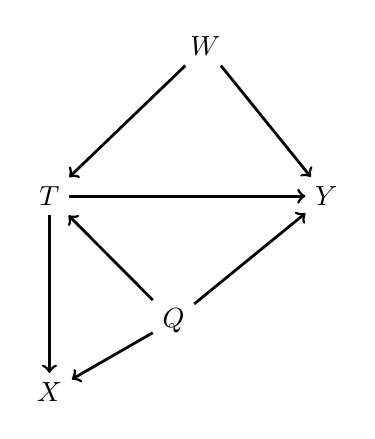
\begin{tikzpicture}
		% nodes %
		\node[text centered] (t) {$T$};
		\node[below = 2 of t, text centered] (b) {$X$};
		\node[right=3 of t, text centered] (y) {$Y$};
		\node[above right=2 of t, text centered] (a) {$W$};
		\node[below right=1.5 of t, text centered] (c) {$Q$};
		
		
		% edges %
		\draw[->, line width= 1] (t) --  (y);
		\draw[->, line width= 1] (t) --  (b);
		\draw[->, line width= 1] (c) --  (t);
		\draw[->, line width= 1] (c) --  (y);
		\draw[->, line width= 1] (a) --  (t);
		\draw[->, line width= 1] (a) --  (y);
		\draw[->, line width= 1] (c) --  (b);
	\end{tikzpicture}
\end{figure}

\FloatBarrier

\paragraph*{Q1a}
Assume that you are interested in the relationship between $T$ and $Y$ and that $T$ only takes values of zero or one. What would happen if you chose to estimate this relationship by comparing the sample average of $Y$ among observations where $T=1$ to the sample average of $Y$ among observations where $T=0$? 


\vspace{2cm}

\paragraph*{Q1b}
Using conditional expectations, write out the ideal comparison to identify the relationship between $T$ and $Y$.


\clearpage

\section*{Q2 - Calculating Probabilities with Known Distributions}

\paragraph*{Q2a}

Consider a random variable $X$, where $X \sim N(0,1)$. Use R to find $Pr(X \leq 1.64)$.

\vspace{2cm}

\paragraph*{Q2b}

Consider a random variable $X$, where $X \sim N(42,8)$. Use R to find $Pr(X \geq 30)$.

\vspace{2cm}

\paragraph*{Q2c}
Consider a random variable $X$, where $X \sim N(0,1)$. Use R to find $Pr(|X| \geq 1.64)$.

\vspace{2cm}

\paragraph*{Q2d}
Consider a random variable $X$, where $X \sim N(0,1)$. Use R to find $Pr(X \leq -1.64 \cup X \geq 2.5)$.

\vspace{2cm}

\clearpage


\section*{Q3 - The Age of UMaine Students}

Download the ``E2data.RData'' data set and load it in R. Assume that the observations in the \textit{universe} data frame represent the entire population of UMaine students. Assume that the true average age ($\mu$) of a UMaine student is 22.

\vspace{.25cm}

\paragraph*{Q3a}
Consider the three estimators proposed below. Show whether each estimator is unbiased. Which one is the most efficient?

\begin{itemize}
	\item $\bar{y} = \frac{\sum_{i=1}^n y_i}{n}$
	\item $\tilde{y} = \frac{\sum_{i=1}^{5} y_i}{5}$
	\item $\hat{y}=y_1$ (The first observation you draw)
\end{itemize} 

\vspace{2cm}

\paragraph*{Q3b}
Draw a sample of 25 observations from the \textit{universe} data frame. Using the sample, calculate an estimate of $\mu$ using $\bar{y}$, $\tilde{y}$ and $\hat{y}$. Report your estimates. Which one is the closest to the true value of $\mu$?


\clearpage

\subsection*{Q4 - Hypothesis Testing}

Imagine that you are interested the effect of going on a daily jog ($\bh$) and life expectancy. 

\begin{itemize}
	\item[] You estimate $\bh = 6.25$ after analyzing a sample of 502 observations. 
	\item[] The standard error of your estimate is 1.43. 
\end{itemize}


\paragraph*{Q4a} Test the following null hypotheses against the alternative, assuming you are willing to accept a 5\% chance of committing a Type I error:
\begin{itemize}
	\item[] $H_0: \: \beta=9.25$
	\item[] $H_0: \: \beta=2.1$
	\item[] $H_0: \: \beta=3.5$
\end{itemize}

\vspace{2cm}

\paragraph*{Q4b} Still using the estimate from above, construct the following confidence intervals. Plot the confidence intervals in R and be sure to interpret each interval in words.

\begin{itemize}
	\item[] 95\% Confidence Interval
	\item[] 99\% Confidence Interval
\end{itemize}


\paragraph*{Q4c} What is the smallest sized test for which you would reject the null hypotheses below?

\begin{itemize}
	\item[] $H_0: \: \beta=4$
\end{itemize}



\clearpage

\section*{Q5 - The Effect of Studying Hard on GPA}

In this section, we will return to our assessment of the relationship between studying hard and GPA. Consider the estimator:

$$\hat{\gamma} = \bar{y}_1 - \bar{y}_2 $$

Where:
\begin{itemize}
	\item $\bar{y}_1$ is the average GPA among students who report studying hard.
	\item $\bar{y}_0$ is the average GPA among students who do not report studying hard.
\end{itemize}

The standard error of this estimator can be calculated as:

$$ se(\hat{\gamma}) = \sqrt{ \frac{s^2_1}{n_1}+\frac{s^2_0}{n_0}}$$

Where:
\begin{itemize}
	\item $s^2_1$ is the sample variance of GPA among students who study hard.
	\item $n_1$ is the number of students who study hard.
	\item $s^2_0$ and $n_0$ are similarly defined for students who did not study hard.
\end{itemize}

\clearpage

\paragraph*{Q5a -} Using the full sample, calculate an estimate of $\hat{\gamma}$.

\vspace{2cm}

\paragraph*{Q5b -} Calculate the standard error associated with your estimate.

\vspace{2cm}

\paragraph*{Q5c -} Test the hypothesis that studying hard has no effect on GPA

\vspace{2cm}

\paragraph*{Q5d -} Construct and discuss a 95 \% confidence interval around your estimate of $\hat{\gamma}$


\clearpage

\vspace{2cm}

\section*{Q6...Conditional on the library}

Repeat the tasks from \textbf{Q5a}, \textbf{Q5b}, and \textbf{Q5d}, but this time focus only on students who know where the library is. Compare and contrast your results to those you obtained in \textbf{Q5}.






\end{document}	%End document